\documentclass{simplesnt}

%% Helpful packages
\usepackage{simplebnf}[2023/11/25]
\usepackage{kotex}

\usepackage{listings}
\lstset{basicstyle = \small\ttfamily, breaklines}

\usepackage{tabularray}
\UseTblrLibrary{booktabs}

\usepackage{metalogo} % For XeTeX logo
\usepackage{kotex-logo}

\newcommand*{\presentfont}[1]{{\fontspec{#1}#1}}
\ExplSyntaxOn
\bool_if:nF { \sys_if_engine_xetex_p: || \sys_if_engine_luatex_p: }
  { \newcommand*{\fontspec}[1]{} }
\ExplSyntaxOff

\title{\texttt{분석기 취약점 파고들기}}
\author{정원준}

\begin{document}
\date{2025년 8월 8일}
\maketitle


\begin{frame}
  \frametitle{목차}
  \tableofcontents
\end{frame}


\section{정적 분석이 무엇인가}

\begin{frame}[c, fragile]
  \frametitle{문제 상황}

  \setlength{\columnsep}{10pt}

  \begin{columns}[T]
    \column{0.5\textwidth}
    \lstset{
      language=Python,
      basicstyle=\ttfamily\small,
      lineskip=2pt,
      columns=fullflexible,
    }
    \begin{lstlisting}
x = int(input())

while x > 1:
    if x % 2 == 0:
        x = x//2
    else:
        x = 3*x + 1

print(x)
    \end{lstlisting}

    \column{0.5\textwidth}
    \vspace{8pt}
    \begin{itemize}
      \item x가 어떤 값을 가질 수 있을까?
      \item x가 특정 위치에서 어떤 값을 가질 수 있을까?
    \end{itemize}
  \end{columns}

\end{frame}

\begin{frame}[c, fragile]
  \frametitle{놓침없이 따지기}
  
  \begin{columns}[T] % T는 상단 정렬
    \column{0.55\textwidth}
    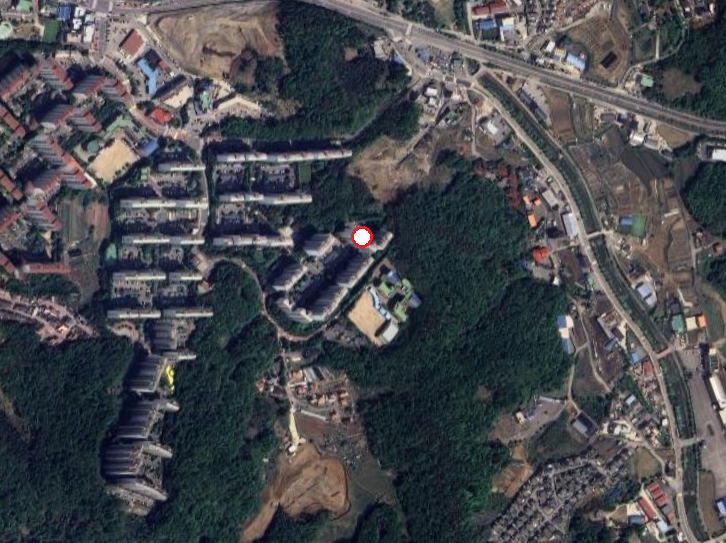
\includegraphics[width=\linewidth]{img/위성지도.png}

    \column{0.45\textwidth}
    {\raggedleft
    ``엄마 놀러갔다 올게요''
    }
    
    \vspace{1.5em}
    
    {\centering
    \small \textit{10분 뒤..} \par
    }
    
    \vspace{1.5em}
    
    {\raggedleft
    `우리 애가 어디쯤 있을까?'
    }

  \end{columns}
\end{frame}

\begin{frame}[c, fragile]
  \frametitle{놓침없이 따지기}
  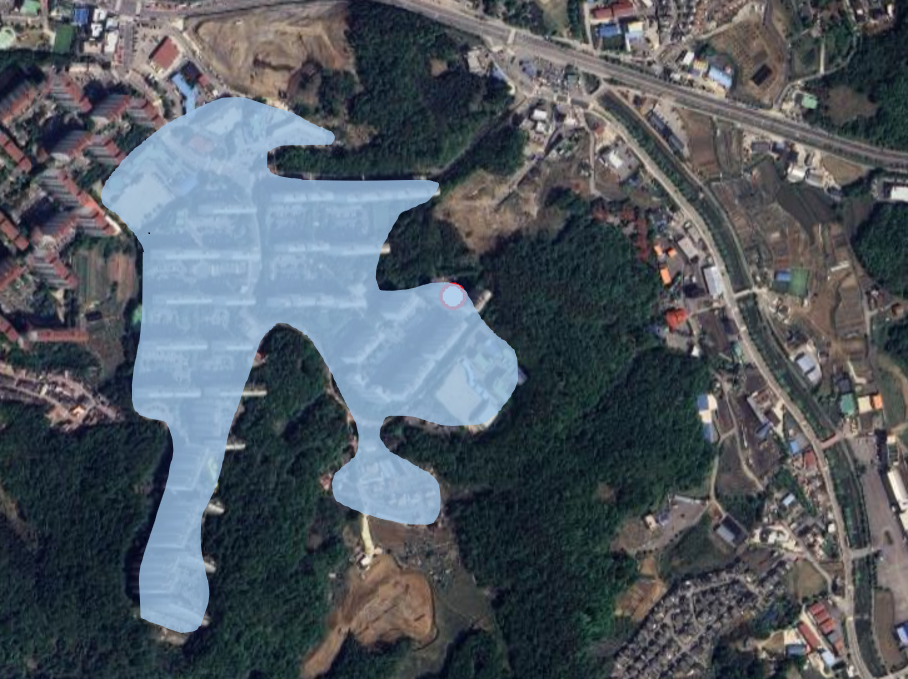
\includegraphics[width=\linewidth]{img/가능지역.png}
\end{frame}


\begin{frame}[c, fragile]
  \frametitle{놓침없이 따지기}
  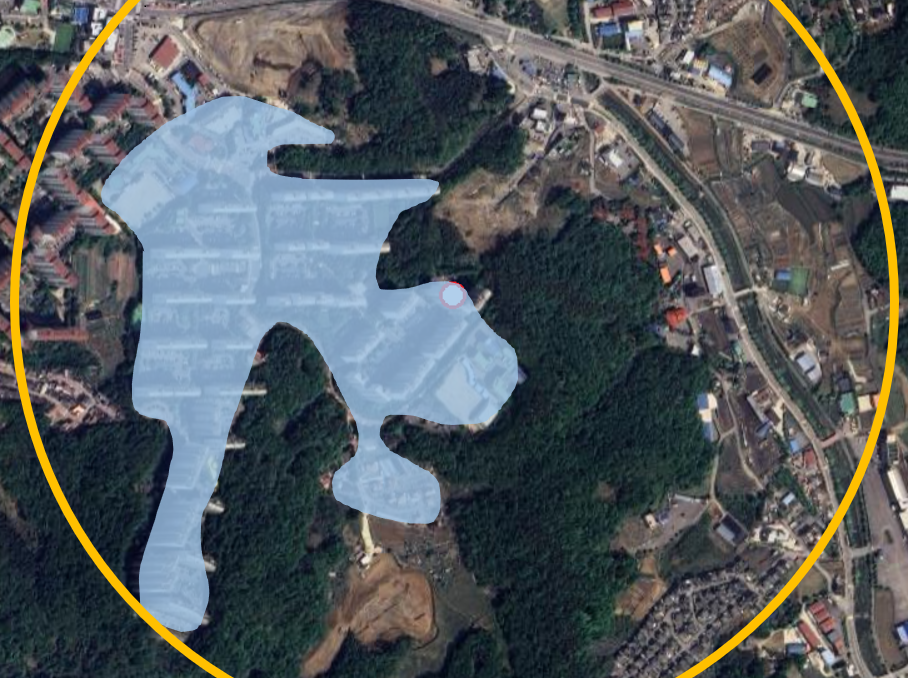
\includegraphics[width=\linewidth]{img/놓침없이따지는.png}
\end{frame}

\section{걱정거리}


\begin{frame}[c, fragile]
\end{frame}
\begin{frame}[c, fragile]
\end{frame}
\begin{frame}[c, fragile]
\end{frame}

\section{공격의 기대효과}

\begin{frame}[c, fragile]
\end{frame}
\begin{frame}[c, fragile]
\end{frame}

\section{마저 할 일}

\begin{frame}[c, fragile]
\end{frame}
\begin{frame}[c, fragile]
\end{frame}

\end{document}
